\documentclass[a4paper,12pt]{report}

% Packages
\usepackage{graphicx} % for including images
\usepackage{amsmath} % for math symbols
\usepackage{geometry} % to set page margins
\geometry{top=1in, bottom=1in, left=1in, right=1in}
\usepackage{listings}
\usepackage{xcolor}

% Define Verilog style for lstlisting
\lstdefinelanguage{Verilog}{
    keywords=[1]{module, input, output, wire, reg, assign, always, if, else, case, endcase, begin, end, localparam, posedge, negedge},
    keywordstyle=\color{blue}\bfseries,
    morekeywords=[2]{posedge, negedge, inout},
    keywordstyle=[2]\color{purple}\bfseries,
    identifierstyle=\color{black},
    sensitive=true,
    morecomment=[l]{//},
    morestring=[b]",
    commentstyle=\color{gray}\ttfamily,
    stringstyle=\color{orange}\ttfamily,
    basicstyle=\ttfamily\footnotesize,
    showstringspaces=false,
    numbers=left,
    numberstyle=\tiny\color{gray},
    stepnumber=1,
    numbersep=5pt,
    frame=single,
    rulecolor=\color{black},
    breaklines=true,
    columns=fullflexible,
    escapeinside={(*@}{@*)}
}

% Title Page
\title{
    \vspace{2in}
    \Huge \textbf{Verilog Implementation of I2C Protocol} \\
    \vspace{1in}
    
\includegraphics[width=0.3\textwidth]{nitc_logo.png} \\
    \Large \textbf{National Institute of Technology Calicut} % Decreased size of college name
    \vspace{0.5in}
}

\author{
    \Large \textbf{Dr. Ashutosh Mishra} \\[0.2cm] 
    \normalsize Professor, ECED\\
    \normalsize National Institute of Technology Calicut, Kerala, India \\[0.5cm]
    \textbf{Project by:} \\[0.5cm]
    \begin{tabular}{c c}
        \textbf{Jagadeesh Mummana} & \textbf{Yasaswi Akkineni} \\[0.2cm]
        (B231113EC) & (B231347EC) \\[0.5cm] % Roll numbers
    \end{tabular}
    \\[0.5cm] 
    \textbf{Department of Electronics and Communication Engineering} \\[0.2cm]
    \textbf{Semester:} III \\[0.2cm]
    \textbf{Course:} Elective - EC2024E Hardware Modelling using HDL
}
\date{}


\begin{document}

% Title page
\maketitle
\clearpage

% Table of Contents
\tableofcontents
\clearpage

% Overview Section
\chapter{Overview}
\section{Project Abstract}
This project focuses on the \textbf{Verilog implementation of the I2C (Inter-Integrated Circuit) protocol}, a widely used serial communication standard that allows multiple devices to communicate over just two wires. I2C is designed to be both \textbf{simple and efficient}, making it ideal for embedded systems that connect low-speed peripherals such as sensors, EEPROMs, and microcontrollers. The goal of this project is to develop a Verilog model that accurately simulates the I2C protocol, enabling multiple devices to exchange data on a shared communication line while showcasing the flexibility and effectiveness of Verilog in hardware design.

\section{Background and Motivation}
Communication protocols are vital in embedded systems, facilitating reliable and efficient data exchange between devices. Among various protocols, \textbf{I2C stands out for its simplicity and capacity to support multiple devices using only two wires}. In contrast to protocols like SPI, which require more connections for multi-device configurations, I2C’s minimal wiring makes it particularly suitable for \textbf{space-constrained applications and cost-effective designs}. This flexibility makes I2C a preferred choice in systems where effective communication between components is essential.

% Project Proposal Section
\chapter{Project Proposal}
\section{Project Description}
This project focuses on the \textbf{Verilog implementation of the I2C (Inter-Integrated Circuit) protocol}, a popular communication method used in embedded systems. Communication protocols are essential because they define the rules and conventions for data exchange between devices. I2C stands out by combining the best features of other protocols like \textbf{SPI (Serial Peripheral Interface)} and \textbf{UART (Universal Asynchronous Receiver-Transmitter)}. With I2C, multiple slave devices can be connected to a single master device, allowing for efficient data sharing. Moreover, it supports multiple masters, enabling several controllers to communicate with one or more slaves. This capability is particularly beneficial in applications where multiple microcontrollers need to log data to a single memory card or display information on a single LCD. Our project aims to create a Verilog model that accurately simulates the I2C protocol, demonstrating how these devices can communicate effectively and showcasing Verilog's utility in hardware design.

\newpage

\section{Intro to Inter-Integrated Circuit Protocol}
\subsection{Comparison with Other Communication Protocols}
\subsection*{Industrial Applications of I\textsuperscript{2}C Protocol}

The Inter-Integrated Circuit (I\textsuperscript{2}C) protocol is a widely used serial communication standard in industrial environments, valued for its simplicity, cost-effectiveness, and minimal wiring requirements. It is ideal for short-distance communication and low-power applications, making it well-suited for industrial settings. Key industrial applications of I\textsuperscript{2}C are outlined below.

\subsubsection*{Sensor Integration and Monitoring}
I\textsuperscript{2}C is commonly used to connect various sensors to a central processor or microcontroller, enabling real-time data acquisition essential for industrial automation and control.
\begin{itemize}
    \item \textbf{Temperature, Humidity, and Pressure Sensors}: These sensors monitor environmental conditions in factories, data centers, and storage facilities. I\textsuperscript{2}C enables multiple sensors to communicate with a central controller, which processes data to maintain optimal conditions.
    \item \textbf{Vibration and Motion Sensors}: Used for predictive maintenance, these sensors monitor machinery health. I\textsuperscript{2}C communication with a central processor allows for data analysis, enabling detection of wear or impending failures to reduce unplanned downtime.
    \item \textbf{Gas and Chemical Sensors}: In chemical plants, gas sensors detect harmful gases and leaks. I\textsuperscript{2}C facilitates communication with a monitoring system, ensuring quick detection and response to hazardous conditions.
\end{itemize}

\subsubsection*{Industrial Control Systems}
I\textsuperscript{2}C is used extensively in industrial control systems to enable efficient communication between modules and controllers.
\begin{itemize}
    \item \textbf{Programmable Logic Controllers (PLCs)}: I\textsuperscript{2}C interfaces with peripheral modules like ADCs and DACs in PLC systems, converting analog sensor signals into digital data for automation and control.
    \item \textbf{Motor Controllers}: In robotics, conveyor belts, and automated machinery, I\textsuperscript{2}C is used for communication between motor controllers and the CPU, allowing precise control of speed, position, and torque.
    \item \textbf{Human-Machine Interfaces (HMIs)}: I\textsuperscript{2}C connects small displays to control units in industrial equipment, allowing real-time system visualization and updates for operators.
\end{itemize}

\subsubsection*{Data Acquisition Systems}
Data acquisition, crucial in industrial quality control and process monitoring, benefits from I\textsuperscript{2}C’s ability to connect multiple sensors or data modules to a single controller with minimal wiring.
\begin{itemize}
    \item \textbf{Analog-to-Digital and Digital-to-Analog Converters}: I\textsuperscript{2}C interfaces ADCs and DACs with a central processor to process analog data from sensors for real-time decision-making.
    \item \textbf{Data Logging and Memory Modules}: Data loggers and memory modules connected over I\textsuperscript{2}C allow periodic data storage, crucial for monitoring environments in factories or energy usage in power plants.
\end{itemize}

\subsubsection*{Industrial Communication and Diagnostics}
I\textsuperscript{2}C supports diagnostic applications in industrial systems, allowing engineers to monitor and troubleshoot components.
\begin{itemize}
    \item \textbf{Diagnostic Modules}: Diagnostic modules using I\textsuperscript{2}C enable real-time tracking of equipment health and quick detection of issues through communication with a central processor.
    \item \textbf{Firmware Updates and Calibration}: I\textsuperscript{2}C enables in-field updates and recalibration by interfacing with memory chips that store configuration and calibration data for industrial devices.
\end{itemize}

\subsubsection*{Battery-Operated and Low-Power Industrial Devices}
In remote or battery-operated equipment, where low power is essential, I\textsuperscript{2}C’s efficiency makes it ideal.
\begin{itemize}
    \item \textbf{Portable Measurement Instruments}: Handheld tools, such as digital multimeters, use I\textsuperscript{2}C to connect internal components (e.g., displays, sensors) while minimizing power consumption.
    \item \textbf{Battery Management Systems (BMS)}: In applications like electric vehicles, BMSs use I\textsuperscript{2}C to monitor battery health, charge, and discharge cycles, ensuring efficient energy management.
\end{itemize}

\textbf{Conclusion}: I\textsuperscript{2}C’s capability to connect multiple devices on a single bus with minimal wiring, along with its low power requirements, makes it an ideal protocol for various industrial applications. From sensor integration to control systems and data acquisition, I\textsuperscript{2}C offers a reliable and cost-effective solution for modern industrial automation and monitoring.
\newpage 
To understand the advantages of communicating over I2C, it's essential to compare it with other available options, particularly \textbf{UART} and \textbf{SPI}.

\vspace{0.25in}

\textbf{Limitations of Serial UART Ports:}  
Serial UART ports are asynchronous, meaning they do not transmit clock data alongside the information. As a result, the devices must agree in advance on a data rate, and their clocks need to maintain close synchronization. Any significant discrepancy in clock rates can lead to garbled data. Moreover, asynchronous serial ports require substantial hardware overhead; the UART implementation at each end is relatively complex and challenging to accurately realize in software. Each frame of data includes at least one start bit and one stop bit, resulting in 10 bits of transmission time for every 8 bits of data, which adversely affects the effective data rate.

\vspace{0.25in}

Furthermore, UART ports are primarily designed for communication between two devices. Although multiple devices can be connected to a single serial port, this leads to \textbf{bus contention}, where multiple devices attempt to drive the same line simultaneously. This contention must be managed to prevent potential damage to the devices, typically requiring additional external hardware. Lastly, while there is no theoretical limit to the data rates of asynchronous serial communications, most UART devices support a limited set of fixed baud rates, typically capping around 230,400 bits per second.

\begin{figure}[htbp]
    \centering
    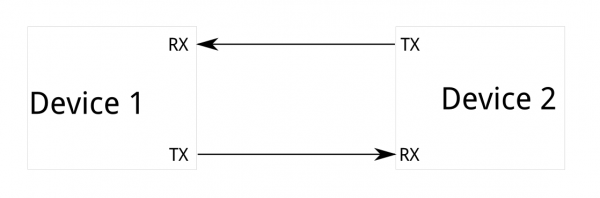
\includegraphics[width=0.8\textwidth]{uart_block_diagram.png} % Replace with actual filename for UART block diagram
    \caption{Block Diagram of an Asynchronous Serial System}
    \label{fig:uart_block_diagram}
\end{figure}

\newpage

\textbf{Drawbacks of SPI:}  
The most significant limitation of the Serial Peripheral Interface (\textbf{SPI}) is the number of pins it requires. Connecting a single controller to one peripheral necessitates four lines; adding each additional peripheral demands an extra chip select I/O pin on the controller. This proliferation of pin connections becomes cumbersome in situations where numerous devices need to connect to a single controller, complicating the routing of signals in constrained PCB layouts. 

\vspace{0.25in}

Additionally, SPI supports only one controller on the bus but can accommodate multiple peripheral devices, limited only by the drive capabilities of the connected devices and the availability of chip select pins. While SPI enables high data rate full-duplex communication (simultaneous sending and receiving of data) with clock rates exceeding 10 MHz, the implementation typically involves simple shift registers, facilitating easier software integration.

\begin{figure}[htbp]
    \centering
    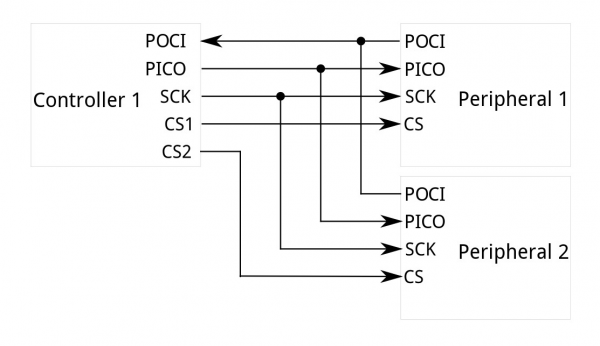
\includegraphics[width=0.8\textwidth]{spi_block_diagram.png} % Replace with actual filename for SPI block diagram
    \caption{Block Diagram of an SPI System}
    \label{fig:spi_block_diagram}
\end{figure}

\newpage

\textbf{The Advantages of I2C:}  
I2C combines the strengths of both UART and SPI. It operates using just two wires, like asynchronous serial, yet supports communication with up to 1,008 peripheral devices. Unlike SPI, I2C accommodates multi-controller systems, allowing more than one controller to communicate with all peripheral devices on the bus (although the controllers must take turns using the bus lines). 

\vspace{0.25in}

I2C data rates fall between those of asynchronous serial and SPI, with most devices communicating at 100 kHz or 400 kHz. While there is some overhead—requiring one additional acknowledgment (ACK/NACK) bit for every 8 bits of data transmitted—I2C remains efficient. Although implementing I2C requires more complex hardware than SPI, it is still simpler than asynchronous serial and can be easily realized in software.

\begin{figure}[htbp]
    \centering
    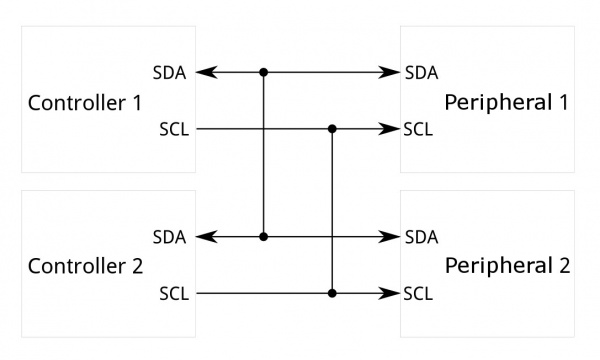
\includegraphics[width=0.8\textwidth]{i2c_block_diagram.png} % Replace with actual filename for I2C block diagram
    \caption{Block Diagram of an I2C System}
    \label{fig:i2c_block_diagram}
\end{figure}


\newpage 

\section{Physical layer}
\subsection{Two-Wire Communication}

An I2C system utilizes \textbf{two shared communication lines} for all devices on the bus. These two lines facilitate \textbf{bidirectional, half-duplex communication}. I2C supports multiple controllers and multiple target devices, making it a flexible choice for various applications. It is essential to use \textbf{pull-up resistors} on both of these lines to ensure proper operation. Fig \ref{fig:i2c_implementation} shows a typical implementation of the I2C physical layer.
\vspace{0.25in}
\begin{figure}[htbp]
    \centering
    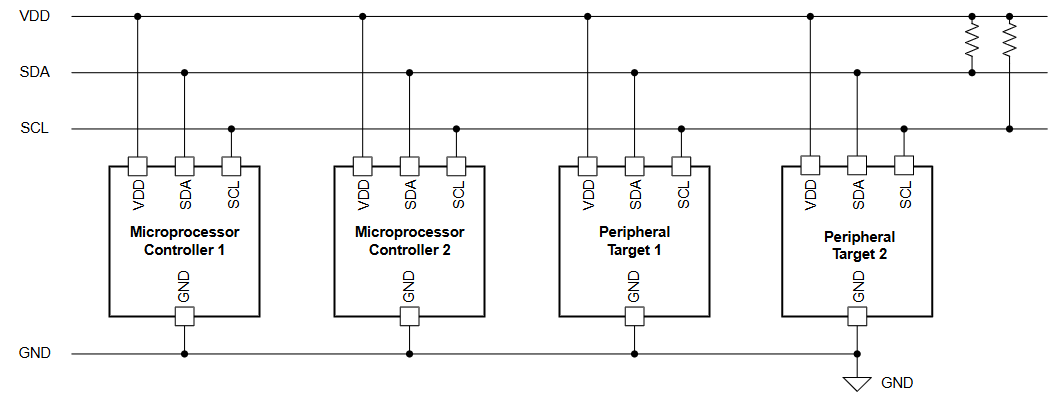
\includegraphics[width=0.8\textwidth]{i2c_physical_layer.png} % Change the filename to your actual image filename
    \caption{Typical I2C Implementation}
    \label{fig:i2c_implementation}
\end{figure}


One of the main reasons that I2C is a widely adopted protocol is due to its requirement of only \textbf{two lines} for communication. The first line, \textbf{SCL}, is the serial clock line, primarily controlled by the controller device. SCL is responsible for synchronously clocking data in or out of the target device. The second line, \textbf{SDA}, is the serial data line, used to transmit data to or from the target devices. For instance, a controller device can send configuration data and output codes to a target \textbf{digital-to-analog converter (DAC)}, or a target \textbf{analog-to-digital converter (ADC)} can send conversion data back to the controller device.

\vspace*{0.25in}

I2C operates as a \textbf{half-duplex communication} protocol, meaning that only one controller or target device can send data on the bus at any given time. In contrast, the \textbf{Serial Peripheral Interface (SPI)} is a \textbf{full-duplex protocol} that allows data to be sent and received simultaneously, requiring four lines for communication: two data lines for sending and receiving data, along with a serial clock and a unique SPI chip select line to select the device for communication.

\vspace{0.25in}

An I2C controller device initiates and terminates communication, which eliminates potential issues related to \textbf{bus contention}. Communication with a target device is established through a \textbf{unique address} on the bus, allowing multiple controllers and multiple target devices to coexist on the I2C bus.

\vspace{0.25in}

The SDA and SCL lines have an \textbf{open-drain connection} to all devices on the bus, necessitating a pull-up resistor connected to a common voltage supply.

\subsection{Open-Drain Connection}

The \textbf{open-drain connections} are employed on both the SDA and SCL lines and are linked to an NMOS transistor. This open-drain configuration manages the I2C communication line by either pulling the line low or allowing it to rise to a high state. The term "open-drain" refers to the NMOS bus connection when the NMOS is turned \textbf{OFF}. Figure \ref{fig:open_drain_connection} illustrates the open-drain connection when the NMOS is turned \textbf{ON}.

\begin{figure}[htbp]
    \centering
    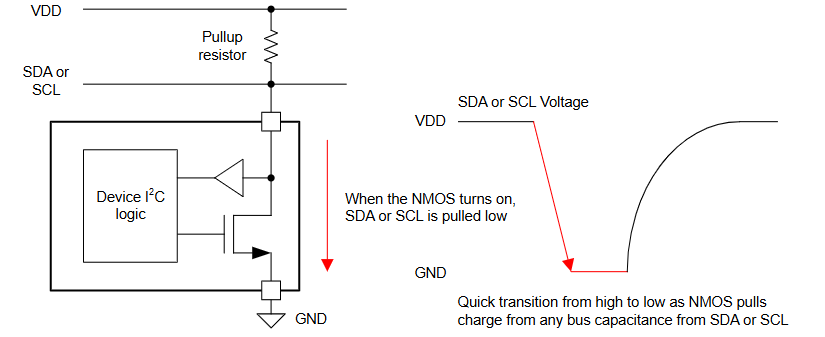
\includegraphics[width=0.8\textwidth]{open_drain_connection.png} % Change the filename to your actual image filename
    \caption{Open-Drain Connection Pulls Line Low When NMOS is Turned On}
    \label{fig:open_drain_connection}
\end{figure}


To establish the voltage level of the SDA or SCL line, the NMOS transistor is either switched \textbf{ON} or \textbf{OFF}. When the NMOS is \textbf{ON}, it allows current to flow through the resistor to ground, effectively pulling the open-drain line low. This transition from high to low is typically rapid, as the NMOS quickly discharges any capacitance on the SDA or SCL lines.

\vspace{0.25in}

When the NMOS turns \textbf{OFF}, the device ceases to pull current, and the pull-up resistor subsequently raises the SDA or SCL line back to \textbf{VDD}. Figure \ref{fig:open_drain_off} shows the open-drain line when the NMOS is turned \textbf{OFF}, illustrating how the pull-up resistor brings the line high.

\begin{figure}[htbp]
    \centering
    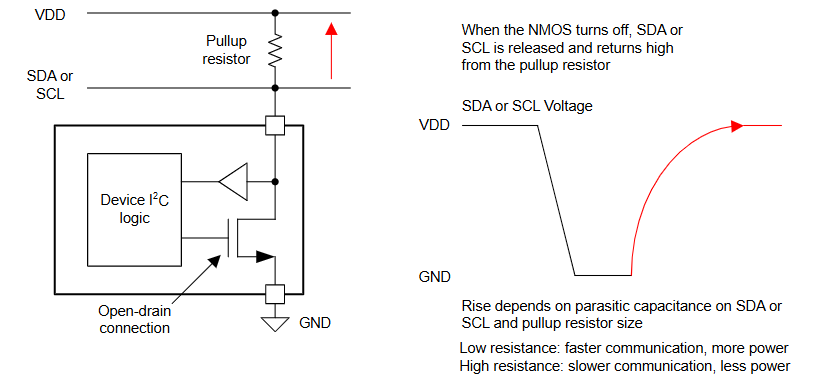
\includegraphics[width=0.8\textwidth]{open_drain_off.png} % Change the filename to your actual image filename
    \caption{Open-Drain Line with NMOS Turned Off}
    \label{fig:open_drain_off}
\end{figure}


The transition of the open-drain line to a high state is slower because the line is pulled up against the bus capacitance, rather than being actively driven high.

\section{I2C Protocol}

Communication over \textbf{I2C} requires a specific signaling protocol to ensure that devices on the bus recognize valid I2C transmissions. While this process is more intricate than \textbf{UART} or \textbf{SPI}, most I2C-compatible devices handle the finer protocol details internally, allowing developers to focus primarily on data exchange.

\vspace{0.25in}

\textbf{SDA and SCL Lines:}  
The I2C bus operates with two main lines: \textbf{SDA} (Serial Data Line) and \textbf{SCL} (Serial Clock Line). Data is transmitted over the \textbf{SDA} line in sync with clock pulses on the \textbf{SCL} line. Generally, data is placed on \textbf{SDA} when \textbf{SCL} is low, and devices sample this data when \textbf{SCL} goes high. If needed, multiple internal \textbf{registers} may control data handling, especially in complex devices.

\vspace{0.25in}

\textbf{Protocol Components:}

\vspace{0.25in}

1. \textbf{Start Condition:}  
   To initiate communication, the controller sets \textbf{SCL} high and then pulls \textbf{SDA} low. This signals all peripheral devices on the bus that a transmission is starting. In cases where multiple controllers attempt to start communication simultaneously, the first device to pull \textbf{SDA} low gains control. If necessary, the controller can issue repeated start conditions to maintain bus control without releasing it.

   \vspace{0.25in}


2. \textbf{Address Frame:}  
   Every I2C transmission begins with an \textbf{address frame} to specify the target peripheral. This frame consists of a 7-bit address, sent \textbf{MSB} (most significant bit) first, followed by a \textbf{R/W bit} indicating the operation type (read or write).  

   \vspace{0.25in}

   After this, the 9th bit, known as the \textbf{ACK/NACK bit}, is used by the receiving device to confirm reception. If the device pulls \textbf{SDA} low before the 9th clock pulse (\textbf{ACK}), communication continues. If not (\textbf{NACK}), it indicates either unrecognized data or an issue in reception, prompting the controller to decide the next steps.

\vspace{0.25in}

3. \textbf{Data Frames:}  
   Following the address frame, one or more \textbf{data frames} are sent over the \textbf{SDA} line. Each data frame is 8 bits, and data is transferred from the controller to the peripheral or vice versa, based on the \textbf{R/W bit} in the address frame.
   
   \vspace{0.25in}

   Many peripheral devices have auto-incrementing \textbf{internal registers}, enabling data to continue from consecutive registers without the need to re-specify the register address.

\vspace{0.25in}

4. \textbf{Stop Condition:}  
   The controller ends communication by generating a \textbf{stop condition}. This is done by transitioning \textbf{SDA} from low to high after a high-to-low transition on \textbf{SCL}, with \textbf{SCL} held high during the stop sequence. To avoid false stop conditions, the value on \textbf{SDA} should not change while \textbf{SCL} is high during regular data transmission.

The \textbf{I2C protocol} divides communication into structured \textbf{frames}. Each communication sequence begins with a \textbf{START} condition, initiated by the controller, followed by an \textbf{address frame} and then one or more \textbf{data frames}. Every frame also includes an acknowledgment (ACK) bit, signaling that the frame has been received successfully by the intended device. \textbf{Figure 3-3} illustrates the structure of two I2C communication frames, showing both address and data frames in detail.

\begin{figure}[htbp]
    \centering
    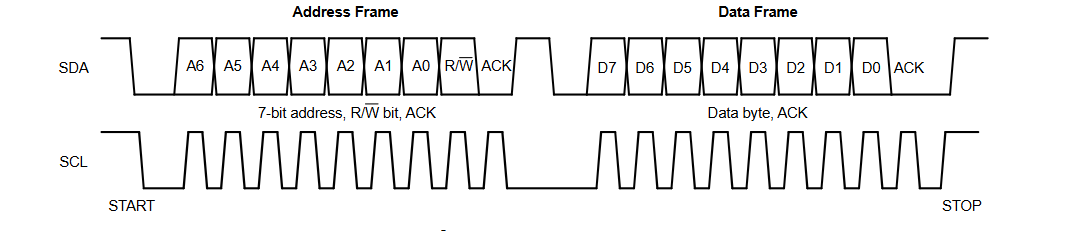
\includegraphics[width=0.8\textwidth]{i2c_frames.png} % Replace with actual filename for I2C frames diagram
    \caption{I2C Address and Data Frames}
    \label{fig:i2c_frames}
\end{figure}

In an I2C transaction, the controller first sends a \textbf{START condition} by pulling the \textbf{SDA} line low, followed by the \textbf{SCL} line. This sequence asserts control over the bus, preventing other devices from interfering. Each target device on the I2C bus has a unique \textbf{7-bit address}, allowing the controller to specify which target device it intends to communicate with.

\vspace{0.25in}

Once the address is set on \textbf{SDA} while \textbf{SCL} acts as the clock, the \textbf{8th bit} (R/W bit) indicates the intended operation type: \textbf{read (1)} or \textbf{write (0)}. This initial address and R/W bit are followed by an \textbf{ACK bit}, sent by the target device to confirm receipt. If the target device receives the address successfully, it pulls \textbf{SDA} low during the next \textbf{SCL} pulse, signaling an ACK. If no device acknowledges, the line remains high, signaling a \textbf{NACK}.

\vspace{0.25in}

After the address frame, one or more \textbf{data frames} follow. Each data frame contains 8 bits of data, which are acknowledged (ACK) in the 9th bit. If the data frame is a \textbf{write} operation, the target device pulls \textbf{SDA} low to confirm data receipt. For \textbf{read} operations, the controller pulls \textbf{SDA} low to acknowledge receipt of the data. The presence or absence of the ACK is essential for troubleshooting, as a missing ACK may indicate an addressing error or transmission failure.

\vspace{0.25in}

Finally, the communication ends with a \textbf{STOP condition}, where the controller releases \textbf{SCL} first, followed by \textbf{SDA}. This action releases the I2C bus for other devices to use, completing the communication cycle.

\vspace{0.25in}

This structured protocol allows for the transmission of multiple bytes within one communication sequence. In cases where a target device has multiple internal \textbf{registers}, a write operation can specify the register to read or write data to, enhancing flexibility and enabling complex data transactions.


\chapter{Module Specifications}
\section{MASTER MODULE}
\subsection{C0d3}

\begin{lstlisting}[language=Verilog, caption={I2C Master Module in Verilog}, label=lst:i2c_master]
`timescale 1ns / 1ps

// Main module declaration
module i2c_master(
    input wire clk,                // System clock
    input wire rst,                // Reset signal
    input wire [6:0] addr,         // 7-bit I2C slave address
    input wire [7:0] data_in,      // Data to send to slave in write mode
    input wire enable,             // Start signal for I2C communication
    input wire rw,                 // Read/Write control (0 for write, 1 for read)
    output reg [7:0] data_out,     // Data received from slave in read mode
    output wire ready,             // Indicates when the master is ready for a new transaction
    inout i2c_sda,                 // I2C data line (SDA) - bidirectional
    inout wire i2c_scl             // I2C clock line (SCL) - bidirectional
);

    // Define states for I2C master FSM
    localparam IDLE = 0;
    localparam START = 1;
    localparam ADDRESS = 2;
    localparam READ_ACK = 3;
    localparam WRITE_DATA = 4;
    localparam WRITE_ACK = 5;
    localparam READ_DATA = 6;
    localparam READ_ACK2 = 7;
    localparam STOP = 8;

    localparam DIVIDE_BY = 4;      // Clock divider to generate I2C clock from system clock

    reg [7:0] state;               // Current state of the FSM
    reg [7:0] saved_addr;          // Stores the 7-bit address and RW bit for the current transaction
    reg [7:0] saved_data;          // Data to be sent in write transactions
    reg [7:0] counter;             // Bit counter for data/address transmission
    reg [7:0] counter2 = 0;        // Divider counter for generating i2c_clk
    reg write_enable;              // Controls whether the master drives SDA line
    reg sda_out;                   // Data to output on SDA line when write_enable is 1
    reg i2c_scl_enable = 0;        // Controls the state of the i2c_scl line (enabled or high)
    reg i2c_clk = 1;               // Internal I2C clock signal

    // Ready signal is high when the master is idle and not in reset
    assign ready = ((rst == 0) && (state == IDLE)) ? 1 : 0;

    // I2C SCL signal: High when i2c_scl_enable is low; otherwise, driven by i2c_clk
    assign i2c_scl = (i2c_scl_enable == 0) ? 1 : i2c_clk;

    // SDA line is driven by sda_out when write_enable is high; otherwise, it's in high-impedance
    assign i2c_sda = (write_enable == 1) ? sda_out : 'bz;

    // I2C clock divider: Divides system clock to generate i2c_clk
    always @(posedge clk) begin
        if (counter2 == (DIVIDE_BY / 2) - 1) begin
            i2c_clk <= ~i2c_clk;    // Toggle i2c_clk when half period is reached
            counter2 <= 0;          // Reset the divider counter
        end else begin
            counter2 <= counter2 + 1; // Increment the divider counter
        end
    end

    // Enable/disable I2C clock based on current state
    always @(negedge i2c_clk or posedge rst) begin
        if (rst == 1) begin
            i2c_scl_enable <= 0;    // Disable SCL on reset
        end else begin
            if ((state == IDLE) || (state == START) || (state == STOP)) begin
                i2c_scl_enable <= 0; // SCL is disabled in IDLE, START, and STOP states
            end else begin
                i2c_scl_enable <= 1; // Enable SCL in other states
            end
        end
    end

    // State machine for controlling the I2C master operation
    always @(posedge i2c_clk or posedge rst) begin
        if (rst == 1) begin
            state <= IDLE;          // Reset state to IDLE on reset
        end else begin
            case (state)
                
                IDLE: begin
                    if (enable) begin
                        state <= START;  // Start I2C transaction when enable is high
                        saved_addr <= {addr, rw};  // Save the 7-bit address and RW bit
                        saved_data <= data_in;     // Save the data to be sent (in write mode)
                    end
                end

                START: begin
                    counter <= 7;          // Initialize bit counter to 7 for 8-bit transmission
                    state <= ADDRESS;      // Move to ADDRESS state
                end

                ADDRESS: begin
                    if (counter == 0) begin 
                        state <= READ_ACK;  // Move to ACK check after sending address and RW bit
                    end else begin
                        counter <= counter - 1;  // Transmit address bits, count down
                    end
                end

                READ_ACK: begin
                    if (i2c_sda == 0) begin  // ACK received (SDA pulled low by slave)
                        counter <= 7;       // Reset bit counter
                        if (saved_addr[0] == 0) state <= WRITE_DATA; // If RW=0, go to write mode
                        else state <= READ_DATA;                     // If RW=1, go to read mode
                    end else begin
                        state <= STOP;      // NACK received, move to STOP state
                    end
                end

                WRITE_DATA: begin
                    if (counter == 0) begin
                        state <= READ_ACK2; // Move to second ACK check after data transmission
                    end else begin
                        counter <= counter - 1; // Transmit data bits, count down
                    end
                end

                READ_ACK2: begin
                    if ((i2c_sda == 0) && (enable == 1)) state <= IDLE; // Return to IDLE on ACK
                    else state <= STOP;  // If NACK received or enable low, go to STOP
                end

                READ_DATA: begin
                    data_out[counter] <= i2c_sda;  // Capture data bit from SDA line
                    if (counter == 0) state <= WRITE_ACK; // After last bit, go to WRITE_ACK
                    else counter <= counter - 1; // Count down for each bit received
                end

                WRITE_ACK: begin
                    state <= STOP;  // Go to STOP after sending ACK
                end

                STOP: begin
                    state <= IDLE;  // Go back to IDLE after STOP condition
                end
            endcase
        end
    end

    // SDA output logic based on the current state
    always @(negedge i2c_clk or posedge rst) begin
        if (rst == 1) begin
            write_enable <= 1;       // Drive SDA high on reset
            sda_out <= 1;
        end else begin
            case (state)
                
                START: begin
                    write_enable <= 1;  // Enable SDA for start condition
                    sda_out <= 0;       // Pull SDA low for start condition
                end
                
                ADDRESS: begin
                    sda_out <= saved_addr[counter]; // Send each bit of the address and RW bit
                end
                
                READ_ACK: begin
                    write_enable <= 0;  // Release SDA to allow slave to drive ACK/NACK
                end
                
                WRITE_DATA: begin 
                    write_enable <= 1;  // Enable SDA for data transmission
                    sda_out <= saved_data[counter]; // Output each bit of data to SDA
                end
                
                WRITE_ACK: begin
                    write_enable <= 1;  // Enable SDA for ACK transmission
                    sda_out <= 0;       // Send ACK by pulling SDA low
                end
                
                READ_DATA: begin
                    write_enable <= 0;  // Release SDA to read data from slave
                end
                
                STOP: begin
                    write_enable <= 1;  // Enable SDA for stop condition
                    sda_out <= 1;       // Release SDA to indicate stop
                end
            endcase
        end
    end

endmodule
\end{lstlisting}
\newpage
\subsection{Explanation}

The provided code is a Verilog implementation of an I2C Master Module. This module enables communication with I2C-compatible devices through the I2C protocol by implementing the necessary operations to generate I2C signals and manage data transfer. Let’s break down each section of the code:

\paragraph{Module Declaration}
The code begins with the module declaration:

\begin{quote}
\begin{verbatim}
module i2c_master(
    input wire clk,               // System clock
    input wire rst,               // Synchronous reset
    input wire [6:0] addr,        // 7-bit I2C address
    input wire [7:0] data_in,     // Data to be transmitted
    input wire enable,            // Enable signal to start I2C transaction
    input wire rw,                // Read/Write control (0 = Write, 1 = Read)
    output reg [7:0] data_out,    // Data received from I2C
    output wire ready,            // Ready signal when module is idle
    inout i2c_sda,                // I2C data line (SDA)
    inout wire i2c_scl            // I2C clock line (SCL)
);
\end{verbatim}
\end{quote}

This module contains inputs for the system clock (\texttt{clk}), reset (\texttt{rst}), I2C address (\texttt{addr}), data to be sent (\texttt{data\_in}), an enable signal (\texttt{enable}), and a Read/Write control (\texttt{rw}). It also provides outputs for data received (\texttt{data\_out}), a ready status signal (\texttt{ready}), and bidirectional I2C lines, \texttt{i2c\_sda} and \texttt{i2c\_scl}.

\paragraph{State Machine Definition}
The code defines several states representing stages in the I2C transaction:

\begin{quote}
\begin{verbatim}
localparam IDLE = 0;
localparam START = 1;
localparam ADDRESS = 2;
localparam READ_ACK = 3;
localparam WRITE_DATA = 4;
localparam WRITE_ACK = 5;
localparam READ_DATA = 6;
localparam READ_ACK2 = 7;
localparam STOP = 8;
\end{verbatim}
\end{quote}

Each \texttt{localparam} corresponds to a state in the Finite State Machine (FSM), controlling the I2C protocol flow, including start, address transmission, acknowledgment (ACK) reception, data transfer, and stop condition generation.

\paragraph{Clock Divider}
To generate a slower clock for the I2C operations, a clock divider is implemented:

\begin{quote}
\begin{verbatim}
always @(posedge clk) begin
    if (counter2 == (DIVIDE_BY / 2) - 1) begin
        i2c_clk <= ~i2c_clk;
        counter2 <= 0;
    end else counter2 <= counter2 + 1;
end
\end{verbatim}
\end{quote}

This block toggles \texttt{i2c\_clk} at a lower frequency than the system clock, \texttt{clk}, using a counter \texttt{counter2} with a division factor defined by \texttt{DIVIDE\_BY}.

\paragraph{SDA and SCL Control}
To control the \texttt{i2c\_sda} and \texttt{i2c\_scl} lines based on the module’s state:

\begin{quote}
\begin{verbatim}
assign ready = ((rst == 0) && (state == IDLE)) ? 1 : 0;
assign i2c_scl = (i2c_scl_enable == 0) ? 1 : i2c_clk;
assign i2c_sda = (write_enable == 1) ? sda_out : 'bz;
\end{verbatim}
\end{quote}

\begin{itemize}
    \item \texttt{ready} is high when the reset is inactive and the state is \texttt{IDLE}.
    \item \texttt{i2c\_scl} is either high (idle state) or follows the divided \texttt{i2c\_clk} signal.
    \item \texttt{i2c\_sda} outputs the value of \texttt{sda\_out} when \texttt{write\_enable} is active. When \texttt{write\_enable} is inactive, \texttt{i2c\_sda} goes to high-impedance (\texttt{'bz}) for reading data.
\end{itemize}

\paragraph{Finite State Machine (FSM)}
The FSM controls the I2C communication process, progressing through states based on the I2C protocol requirements:

\begin{quote}
\begin{verbatim}
always @(posedge i2c_clk or posedge rst) begin
    if (rst == 1) begin
        state <= IDLE;
    end else begin
        case (state)
            IDLE: begin
                if (enable) begin
                    state <= START;
                    saved_addr <= {addr, rw};
                    saved_data <= data_in;
                end
            end
            START: begin
                counter <= 7;
                state <= ADDRESS;
            end
            ...
            STOP: begin
                state <= IDLE;
            end
        endcase
    end
end
\end{verbatim}
\end{quote}

Each state corresponds to an I2C operation:
\begin{itemize}
    \item \texttt{IDLE}: Waits for \texttt{enable} signal to initiate communication.
    \item \texttt{START}: Prepares a start condition by asserting \texttt{sda\_out} low.
    \item \texttt{ADDRESS}: Sends the address and R/W bit.
    \item \texttt{READ\_ACK} and \texttt{READ\_ACK2}: Verifies acknowledgment (ACK) from the slave.
    \item \texttt{WRITE\_DATA} and \texttt{WRITE\_ACK}: Transfers data to the slave and waits for ACK.
    \item \texttt{READ\_DATA}: Receives data from the slave.
    \item \texttt{STOP}: Generates a stop condition and returns to \texttt{IDLE}.
\end{itemize}

\paragraph{SDA Output Logic}
The logic for controlling the \texttt{i2c\_sda} line, depending on the FSM state, is implemented as follows:

\begin{quote}
\begin{verbatim}
always @(negedge i2c_clk or posedge rst) begin
    if (rst == 1) begin
        write_enable <= 1;
        sda_out <= 1;
    end else begin
        case (state)
            START: begin
                write_enable <= 1;
                sda_out <= 0;
            end
            ADDRESS: begin
                sda_out <= saved_addr[counter];
            end
            ...
            STOP: begin
                write_enable <= 1;
                sda_out <= 1;
            end
        endcase
    end
end
\end{verbatim}
\end{quote}

\begin{itemize}
    \item In the \texttt{START} state, \texttt{sda\_out} goes low to generate a start condition.
    \item In the \texttt{ADDRESS} and \texttt{WRITE\_DATA} states, \texttt{sda\_out} sends the bits of \texttt{saved\_addr} or \texttt{saved\_data}.
    \item In \texttt{STOP}, \texttt{sda\_out} goes high to signify the end of the transmission.
\end{itemize}

This Verilog module effectively implements an I2C Master communication sequence by controlling the \texttt{i2c\_sda} and \texttt{i2c\_scl} lines according to the I2C protocol.


\section{SLAVE MODULE}
\subsection{C0d3}
\begin{lstlisting}[language=Verilog, caption={I2C Slave Module in Verilog}, label=lst:i2c_slave]
module i2c_slave(
    input [6:0] addr_in,   // Slave address to respond to (dynamic address input)
    inout sda,             // I2C data line (SDA) - bidirectional
    inout scl              // I2C clock line (SCL)
);

    // Define states for the I2C slave FSM
    localparam READ_ADDR = 0;   // State for reading the address from the master
    localparam SEND_ACK = 1;    // State for sending ACK after receiving a matching address
    localparam READ_DATA = 2;   // State for reading data from the master
    localparam WRITE_DATA = 3;  // State for sending data to the master
    localparam SEND_ACK2 = 4;   // State for sending ACK after receiving data from the master

    reg [7:0] addr;             // Register to store the address received from the master
    reg [7:0] counter;          // Bit counter for data/address transmission
    reg [7:0] state = 0;        // Current state of the FSM
    reg [7:0] data_in = 0;      // Register to store data received from the master
    reg [7:0] data_out = 8'b11001100;  // Data to be sent to the master in read mode
    reg sda_out = 0;            // Data to drive onto SDA when write_enable is high
    reg sda_in = 0;             // Register to capture SDA input data
    reg start = 0;              // Flag to indicate the start condition (SDA goes low while SCL is high)
    reg write_enable = 0;       // Controls whether the slave drives the SDA line

    // Tri-state SDA line: driven by sda_out when write_enable is high, otherwise high-impedance
    assign sda = (write_enable == 1) ? sda_out : 'bz;

    // Detect start condition on SDA falling edge when SCL is high
    always @(negedge sda) begin
        if ((start == 0) && (scl == 1)) begin
            start <= 1;           // Set start flag
            counter <= 7;         // Initialize counter to read 8 bits (address or data)
        end
    end

    // Detect stop condition on SDA rising edge when SCL is high
    always @(posedge sda) begin
        if ((start == 1) && (scl == 1)) begin
            state <= READ_ADDR;   // Go to READ_ADDR state to read the address from master
            start <= 0;           // Clear start flag
            write_enable <= 0;    // Release SDA line
        end
    end

    // State machine for I2C slave behavior, triggered on rising edge of SCL
    always @(posedge scl) begin
        if (start == 1) begin     // Only proceed if start condition was detected
            case(state)
                
                READ_ADDR: begin
                    addr[counter] <= sda;      // Capture address bit from SDA
                    if(counter == 0) begin
                        state <= SEND_ACK;     // Move to SEND_ACK after receiving full address
                    end else begin
                        counter <= counter - 1; // Count down to receive 8 bits
                    end
                end
                
                SEND_ACK: begin
                    // Check if received address matches slave address (addr_in)
                    if(addr[7:1] == addr_in) begin
                        counter <= 7;          // Reset bit counter for next data frame
                        // Determine next state based on R/W bit (addr[0])
                        if(addr[0] == 0) begin 
                            state <= READ_DATA; // If R/W=0, master wants to write, go to READ_DATA
                        end else begin
                            state <= WRITE_DATA; // If R/W=1, master wants to read, go to WRITE_DATA
                        end
                    end else begin
                        state <= READ_ADDR;    // Address mismatch, go back to READ_ADDR
                    end
                end
                
                READ_DATA: begin
                    data_in[counter] <= sda;   // Capture data bit from SDA
                    if(counter == 0) begin
                        state <= SEND_ACK2;    // Move to SEND_ACK2 after receiving full byte
                    end else begin
                        counter <= counter - 1; // Count down to receive 8 bits
                    end
                end
                
                SEND_ACK2: begin
                    state <= READ_ADDR;        // Go back to READ_ADDR to listen for next address
                end
                
                WRITE_DATA: begin
                    // Transmit data_out to master one bit at a time
                    if(counter == 0) begin
                        state <= READ_ADDR;    // After last bit, go back to READ_ADDR
                    end else begin
                        counter <= counter - 1; // Count down for each bit sent
                    end
                end
                
            endcase
        end
    end

    // Control SDA output behavior on falling edge of SCL, depending on the state
    always @(negedge scl) begin
        case(state)
            
            READ_ADDR: begin
                write_enable <= 0;           // Release SDA while reading address
            end
            
            SEND_ACK: begin
                sda_out <= (addr[7:1] == addr_in) ? 0 : 1; // Send ACK (low) if address matches, else NACK (high)
                write_enable <= 1;           // Enable SDA to drive ACK/NACK
            end
            
            READ_DATA: begin
                write_enable <= 0;           // Release SDA while reading data
            end
            
            WRITE_DATA: begin
                sda_out <= data_out[counter]; // Send each bit of data_out on SDA
                write_enable <= 1;           // Enable SDA to drive data
            end
            
            SEND_ACK2: begin
                sda_out <= 0;                // Send ACK (low) after receiving data
                write_enable <= 1;           // Enable SDA to drive ACK
            end
        endcase
    end
endmodule
\end{lstlisting}
\newpage
\subsection{Explanation}

The Verilog code presented is for an I2C Slave Module that implements the core logic for an I2C slave device capable of receiving and transmitting data over the I2C protocol. Let’s break down the components of the code and their functionality:

\paragraph{Module Declaration}
The module begins with the declaration of inputs and outputs:

\begin{quote}
\begin{verbatim}
module i2c_slave(
    input [6:0] addr_in,   // Dynamic address input for I2C slave
    inout sda,             // I2C data line (SDA)
    inout scl              // I2C clock line (SCL)
);
\end{verbatim}
\end{quote}

The inputs include a 7-bit address (\texttt{addr\_in}) for the slave device, along with the bidirectional \texttt{sda} and \texttt{scl} lines for data and clock signals respectively.

\paragraph{State Machine Definition}
The I2C protocol relies on a finite state machine (FSM) to control the data transfer sequence. The FSM is represented by five states:

\begin{quote}
\begin{verbatim}
localparam READ_ADDR = 0;
localparam SEND_ACK = 1;
localparam READ_DATA = 2;
localparam WRITE_DATA = 3;
localparam SEND_ACK2 = 4;
\end{verbatim}
\end{quote}

Each state corresponds to a particular phase of the I2C communication:
- \texttt{READ\_ADDR}: Reads the I2C address and R/W bit.
- \texttt{SEND\_ACK}: Sends acknowledgment (ACK) if the address matches.
- \texttt{READ\_DATA}: Receives data from the master.
- \texttt{WRITE\_DATA}: Sends data to the master.
- \texttt{SEND\_ACK2}: Sends a second ACK after data reception.

\paragraph{Internal Registers and Signals}
Several internal registers and signals are declared to support the functionality of the I2C slave:
- \texttt{addr} holds the slave address and R/W bit.
- \texttt{counter} is used to count bits during transmission.
- \texttt{state} holds the current FSM state.
- \texttt{data\_in} and \texttt{data\_out} store the incoming and outgoing data, respectively.
- \texttt{sda\_out} and \texttt{sda\_in} control the data line (SDA).
- \texttt{start} flags the detection of the I2C start condition.
- \texttt{write\_enable} controls whether the slave can drive the SDA line.

\paragraph{SDA Line Control}
The assignment of the \texttt{sda} line is conditional on the \texttt{write\_enable} signal:

\begin{quote}
\begin{verbatim}
assign sda = (write_enable == 1) ? sda_out : 'bz;
\end{verbatim}
\end{quote}

This means that the slave drives the \texttt{sda} line when \texttt{write\_enable} is active, otherwise, the line is in high-impedance state ('bz).

\paragraph{Start and Stop Condition Detection}
The start condition is detected when there is a falling edge on the \texttt{sda} line while the \texttt{scl} line is high, and the stop condition is detected when there is a rising edge on the \texttt{sda} line while \texttt{scl} is high. These conditions trigger transitions in the FSM.

\begin{quote}
\begin{verbatim}
always @(negedge sda) begin
    if ((start == 0) && (scl == 1)) begin
        start <= 1;           // Set start flag
        counter <= 7;         // Initialize bit counter
    end
end

always @(posedge sda) begin
    if ((start == 1) && (scl == 1)) begin
        state <= READ_ADDR;   // Transition to READ_ADDR state
        start <= 0;           // Reset start flag
        write_enable <= 0;    // Disable write
    end
end
\end{verbatim}
\end{quote}

These blocks capture the start and stop conditions and manage the FSM transitions accordingly.

\paragraph{FSM Logic for Data Transfer}
The FSM operates on the rising edge of the \texttt{scl} signal, progressing through various states based on the detected conditions:

\begin{quote}
\begin{verbatim}
always @(posedge scl) begin
    if (start == 1) begin
        case(state)
            READ_ADDR: begin
                addr[counter] <= sda;
                if(counter == 0) state <= SEND_ACK;
                else counter <= counter - 1;
            end
            SEND_ACK: begin
                if(addr[7:1] == addr_in) begin
                    counter <= 7;
                    if(addr[0] == 0) begin 
                        state <= READ_DATA; // If write mode, move to READ_DATA
                    end else state <= WRITE_DATA; // Else move to WRITE_DATA
                end else state <= READ_ADDR;
            end
            ...
        endcase
    end
end
\end{verbatim}
\end{quote}

The state transitions depend on whether the address matches, the R/W bit, and whether data is being read or written. The \texttt{SEND\_ACK} state sends an acknowledgment if the address is correct, while the \texttt{READ\_DATA} and \texttt{WRITE\_DATA} states handle data reception and transmission respectively.

\paragraph{SDA Output Logic}
The logic for controlling the \texttt{sda} output during the FSM states is defined in the following block:

\begin{quote}
\begin{verbatim}
always @(negedge scl) begin
    case(state)
        READ_ADDR: begin
            write_enable <= 0;            // Disable writing during address read
        end
        SEND_ACK: begin
            sda_out <= (addr[7:1] == addr_in) ? 0 : 1;  // Send ACK (0) or NACK (1)
            write_enable <= 1;    
        end
        READ_DATA: begin
            write_enable <= 0;           // Disable writing during data read
        end
        WRITE_DATA: begin
            sda_out <= data_out[counter]; // Output data bit by bit
            write_enable <= 1;
        end
        SEND_ACK2: begin
            sda_out <= 0;                // Send ACK (0) after data reception
            write_enable <= 1;
        end
    endcase
end
\end{verbatim}
\end{quote}

Each state manipulates the \texttt{sda\_out} signal to either send an acknowledgment (ACK) or transmit the data bit by bit. The \texttt{SEND\_ACK} state checks the address match and sends either an ACK or NACK. The \texttt{WRITE\_DATA} state sends the data, while the \texttt{SEND\_ACK2} state sends an ACK after data reception.

\paragraph{Summary}
This Verilog code implements a simple I2C Slave module that can handle basic I2C communication. It includes start/stop condition detection, address matching, data reception, and data transmission using an FSM. The module can receive data from the I2C master, send data to it, and properly acknowledge the master at each step in the communication process.
\newpage
\section{TOP-LEVEL MODULE}
\subsection{C0d3}

\begin{lstlisting}[language=Verilog, caption={Top Module for Integrating I2C Master and Slave}, label=lst:top_module]
`timescale 1ns / 1ps

// Top module to integrate i2c_master and i2c_slave
// Top module to integrate i2c_master and i2c_slave
module top(
    input wire clk,                 // System clock
    input wire rst,                 // Reset signal
    input wire [6:0] addr,          // 7-bit I2C address for the master to communicate with
    input wire [7:0] data_in,       // Data to be sent from the master to the slave
    input wire enable,              // Enable signal to initiate I2C communication
    input wire rw,                  // Read/Write signal (0 = Write, 1 = Read)
    output wire [7:0] data_out,     // Data received by the master from the slave
    output wire ready,              // Signal indicating the master is ready for a new operation
    inout wire i2c_sda,             // I2C data line (SDA) - bidirectional
    inout wire i2c_scl              // I2C clock line (SCL)
);

    // Internal register to store the address the slave will respond to.
    // This is the fixed address of the slave in this example.
    reg [6:0] slave_address = 7'b0101010;  // Example default slave address

    // Instantiate the I2C slave module
    i2c_slave slave_inst (
        .addr_in(slave_address),   // Provide the fixed slave address to the slave instance
        .sda(i2c_sda),             // Connect the slave's SDA line to the top-level SDA
        .scl(i2c_scl)              // Connect the slave's SCL line to the top-level SCL
    );

    // Instantiate the I2C master module
    i2c_master master_inst (
        .clk(clk),                 // Connect the system clock to the master
        .rst(rst),                 // Connect the reset signal to the master
        .addr(addr),               // Provide the I2C address the master should communicate with
        .data_in(data_in),         // Data to be sent to the slave (if writing)
        .enable(enable),           // Enable signal to start the I2C transaction
        .rw(rw),                   // Read/Write signal (0 = Write, 1 = Read)
        .data_out(data_out),       // Data received from the slave (if reading)
        .ready(ready),             // Master ready signal indicating it's idle or ready for a new transaction
        .i2c_sda(i2c_sda),         // Connect the master's SDA line to the top-level SDA
        .i2c_scl(i2c_scl)          // Connect the master's SCL line to the top-level SCL
    );

endmodule
\end{lstlisting}
\newpage
\subsection{Explanation}
\begin{itemize}
    \item The \texttt{top} module connects an I2C master and slave module on shared \texttt{i2c\_sda} and \texttt{i2c\_scl} lines.
    \item The \texttt{slave\_address} register holds a predefined address used by the slave.
    \item The \texttt{i2c\_slave} and \texttt{i2c\_master} modules are instantiated and connected to share the I2C lines and control signals.
\end{itemize}
\newpage
\section{TESTBENCH MODULE}
\subsection{C0d3}
\begin{lstlisting}[language=Verilog, caption={Testbench Module for Top Module}, label=lst:testbench_module]
`timescale 1ns / 1ps

module i2c_controller_tb();

    // Inputs
    reg clk;                  // System clock
    reg rst;                  // Reset signal
    reg [6:0] addr;           // Address for the master to communicate with
    reg [7:0] data_in;        // Data to be sent from the master to the slave
    reg enable;               // Enable signal to start communication
    reg rw;                   // Read/Write control (0 = Write, 1 = Read)

    // Outputs
    wire [7:0] data_out;      // Data received by the master from the slave
    wire ready;               // Ready signal indicating the master is ready for a new operation

    // Bidirectional wires
    wire i2c_sda;             // I2C data line (SDA) - shared between master and slave
    wire i2c_scl;             // I2C clock line (SCL) - shared between master and slave

    // Instantiate the Top Module (Device Under Test - DUT)
    top uut (
        .clk(clk),           // Connect system clock to DUT
        .rst(rst),           // Connect reset signal to DUT
        .addr(addr),         // Connect address input to DUT
        .data_in(data_in),   // Connect data to be sent by master to DUT
        .enable(enable),     // Connect enable signal to DUT
        .rw(rw),             // Connect read/write control to DUT
        .data_out(data_out), // Receive data read by master from DUT
        .ready(ready),       // Receive ready signal from DUT
        .i2c_sda(i2c_sda),   // Connect bidirectional SDA line
        .i2c_scl(i2c_scl)    // Connect bidirectional SCL line
    );

    // Clock generation
    initial begin
        clk = 0;
        forever #1 clk = ~clk;  // Toggle clock every 1 ns to generate a 2 ns period clock (500 MHz)
    end

    // Test sequence to simulate I2C operations
    initial begin
        // Set up VCD file for waveform dumping
        $dumpfile("i2c_controller_tb.vcd");  // Name of the VCD file for waveform output
        $dumpvars(0, i2c_controller_tb);     // Dump all variables in this module for waveform analysis

        // Initialize Inputs
        rst = 1;           // Assert reset to initialize the system
        enable = 0;        // Initially disable communication
        addr = 7'b0000000; // Set an initial address (not used immediately)
        data_in = 8'b0;    // Set initial data (not used immediately)
        rw = 0;            // Set initial operation to write (0 = Write, 1 = Read)

        // Wait for reset to complete
        #10;
        rst = 0;           // Deassert reset after 10 ns to start normal operation

        // Test Case 1: Write operation with matching address (Expect ACK from slave)
        addr = 7'b0101010;       // Set address to match the slave address
        data_in = 8'b10101010;   // Data to be sent to the slave
        rw = 0;                  // Set operation to write
        enable = 1;              // Assert enable to start the I2C communication
        #20 enable = 0;          // Deassert enable after 20 ns to complete the command

        // Wait and observe response (slave should ACK the address and receive data)
        #100;

        // Test Case 2: Write operation with non-matching address (Expect NACK from slave)
        addr = 7'b1111111;       // Set address to a non-matching address for the slave
        data_in = 8'b11001100;   // Different data to be sent to the slave
        rw = 0;                  // Set operation to write
        enable = 1;              // Assert enable to start the I2C communication
        #20 enable = 0;          // Deassert enable after 20 ns

        // Wait and observe response (slave should NACK the address since it does not match)
        #100;

        // Test Case 3: Read operation with matching address (Expect ACK from slave and read data)
        addr = 7'b0101010;       // Set address to match the slave address
        rw = 1;                  // Set operation to read
        enable = 1;              // Assert enable to start the I2C communication
        #20 enable = 0;          // Deassert enable after 20 ns

        // Wait and observe response (slave should ACK the address and send data to master)
        #100;

        #200
        $finish;  // End the simulation after 200 ns
    end

endmodule
\end{lstlisting}
\newpage
\subsection{Explanation}
\begin{itemize}
    \item \texttt{i2c\_controller\_tb}: Testbench module for the \texttt{top} module integrating the master-slave I2C communication.
    \item A clock signal is generated using a continuous \texttt{initial} block.
    \item Test cases:
        \begin{itemize}
            \item \textbf{Test Case 1}: Matches the slave address, expecting an ACK.
            \item \textbf{Test Case 2}: Uses a non-matching address, expecting a NACK.
            \item \textbf{Test Case 3}: Matches the address and tests a read operation.
        \end{itemize}
    \item At the end of the test cases, the simulation finishes with \texttt{\$finish}.
\end{itemize}
\newpage

\chapter{Results}
\begin{figure}[h!]
    \centering
    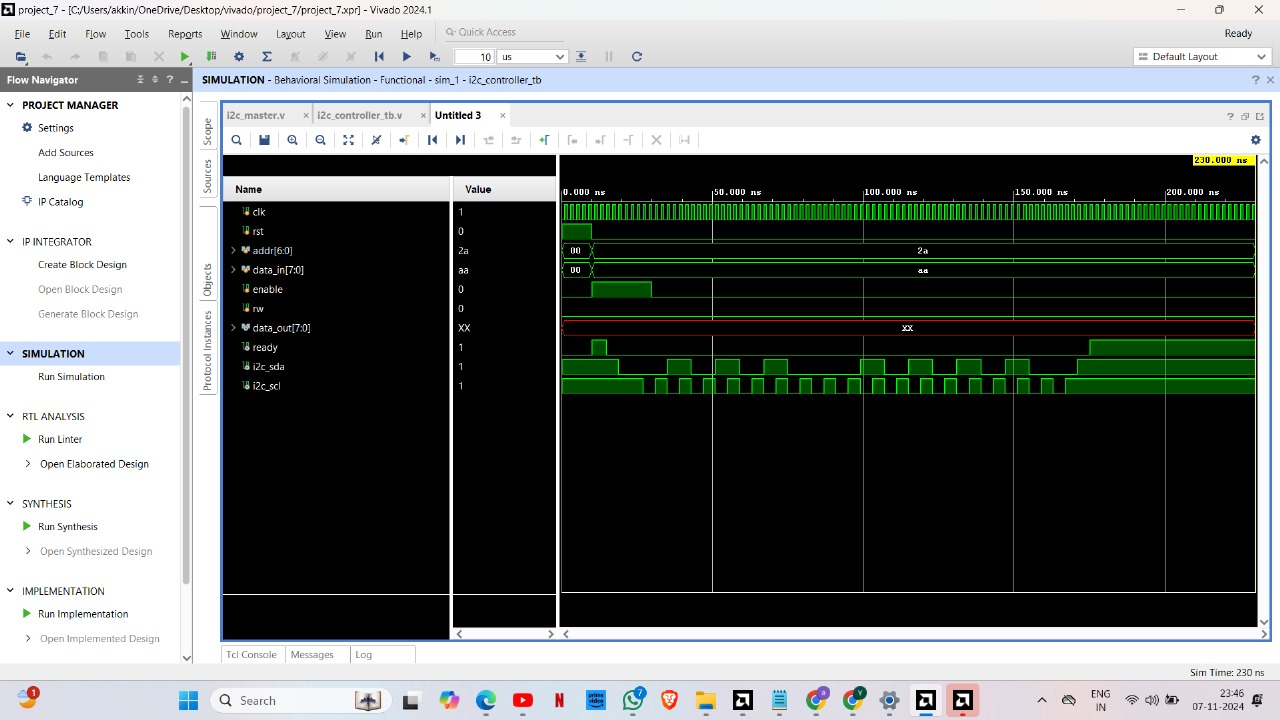
\includegraphics[width=\textwidth]{TEST-CASE-1.jpg}
    \caption{Test Case 1}
\end{figure}
\begin{figure}[h!]
    \centering
    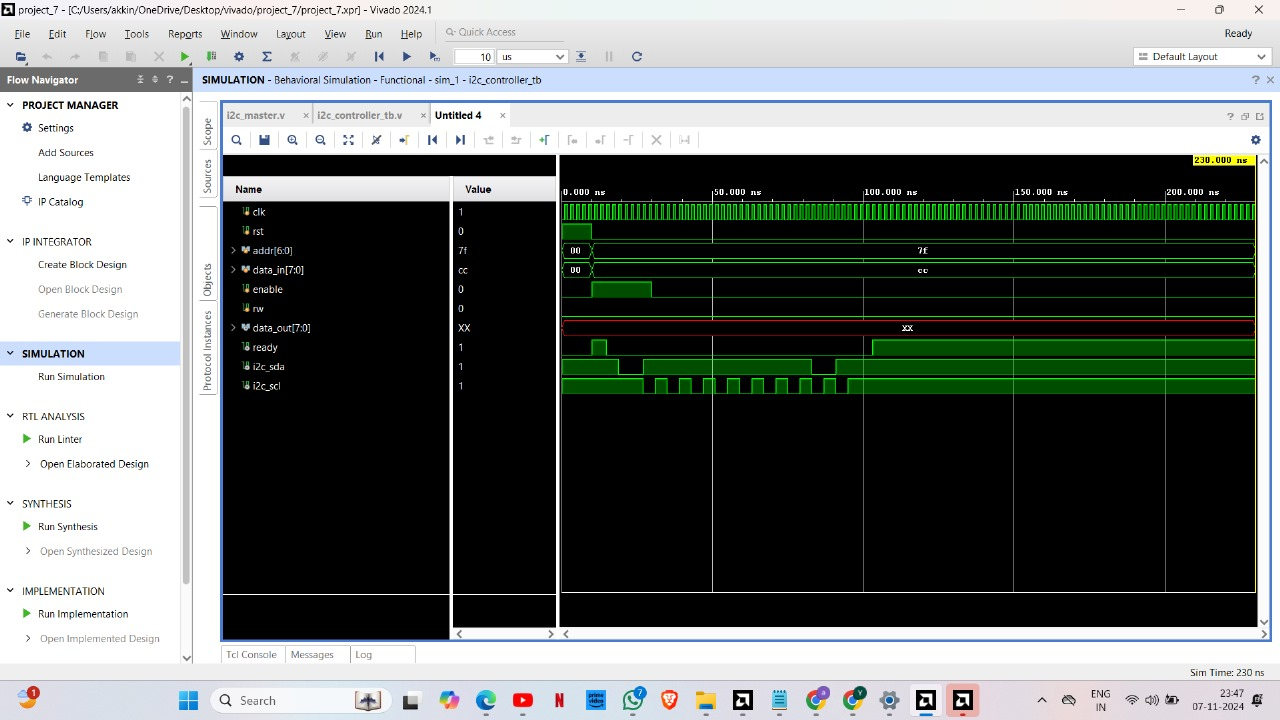
\includegraphics[width=\textwidth]{TEST-CASE-2.jpg}
    \caption{Test Case 2}
\end{figure}

\begin{figure}[h!]
    \centering
    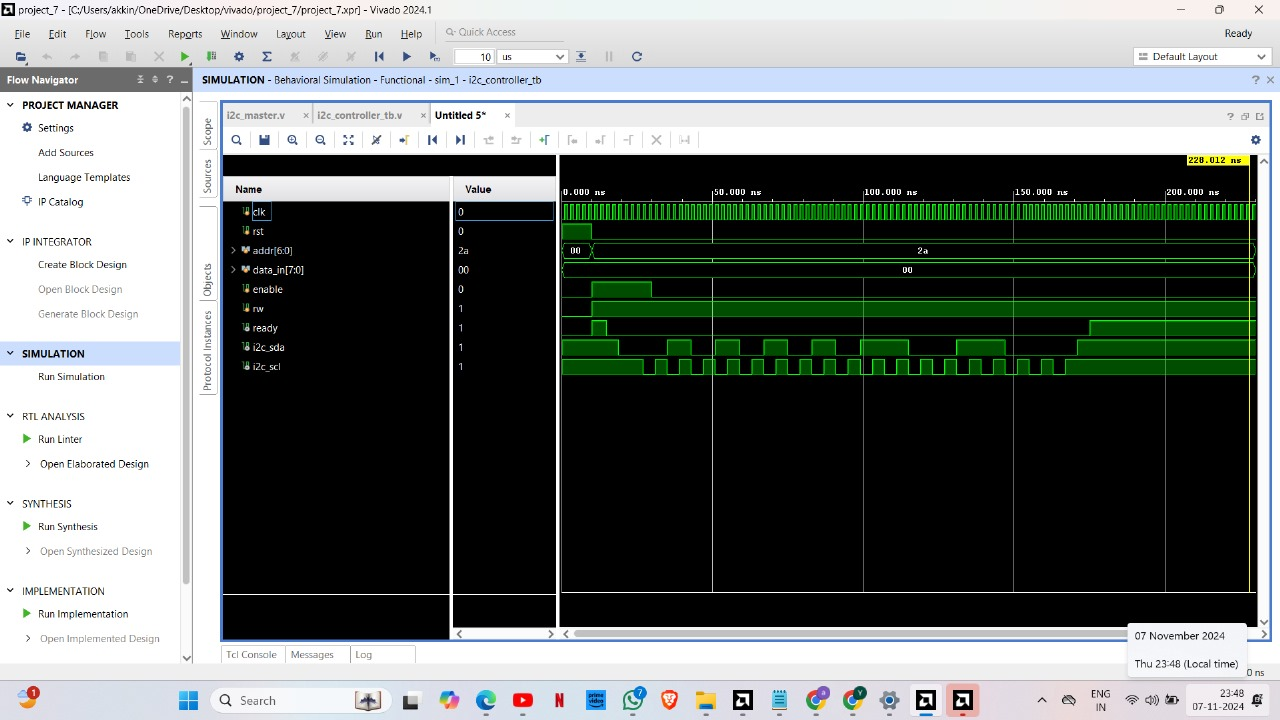
\includegraphics[width=\textwidth]{TEST-CASE-3.jpg}
    \caption{Test Case 3}
\end{figure}
\newpage
\chapter{Challenges and Risk Analysis}

\section{Potential Issues and Solutions}
During the development of our I2C communication project, we encountered several key challenges. Initially, both team members, Jagadeesh and Yasaswi, worked on building basic Verilog modules for the master and slave entities, capable of fundamental read and write functions. Starting with a review of the I2C protocol from online resources and Verilog syntax, we designed a preliminary testbench module. However, as the complexity of the project increased, so did the issues.

\vspace{0.5in}

Yasaswi enhanced the protocol handling by introducing the ACK and NACK flags to manage incorrect slave addresses, as well as refining the finite state machine (FSM) logic for greater robustness. To make the slave module independent of global configurations, we collaboratively designed a top-level module that instantiated both the master and slave modules. This top-level module also verified the slave address, adding an extra layer of validation.

\vspace{0.5in}

Jagadeesh focused on implementing clock stretching between address and data frames to synchronize data transfer. This feature functioned well during address transmissions but revealed discrepancies in the data frame during read operations. We continued troubleshooting this issue, which highlighted the limitations of our initial approach.

\vspace{0.5in}

Eventually, we attempted to implement a multi-master and multi-slave configuration, assigning slave addresses in the format 10101XY (with XY as 00, 01, 10, 11 for slaves 1 through 4) and using a single-bit master select line in the testbench to choose the master. Preloaded data in the slaves was structured as 110011XY to streamline read operations. However, the multi-master configuration still posed unresolved synchronization issues, so we scaled back to a single-master, single-slave model, excluding clock stretching and multiple nodes. Our final implementation focuses on single-point communication, while the initial code attempts and multi-master versions are provided in the appendix via a GitHub link.
\newpage
\section{Risk Management}
Several potential risks arose during the design and integration phases of the project:
\begin{itemize}
    \item \textbf{Design Complexity}: The complexity of the I2C protocol and multi-node configuration presented unforeseen design challenges. Our approach to modular testing helped mitigate issues by allowing iterative refinement.
    \item \textbf{Timing Issues}: Timing mismatches in multi-master configurations posed integration risks, affecting protocol accuracy. This issue is partially resolved in the single-master model but remains a priority for future improvements.
    \item \textbf{FSM Complexity}: Adding ACK/NACK handling increased the FSM complexity, raising the potential for state transition errors. Comprehensive simulation and debugging were essential in minimizing these risks.
\end{itemize}
\newpage
\chapter{Team Contributions and Work Distribution}

\section{Role of Each Team Member}
The project responsibilities were divided between Jagadeesh and Yasaswi, allowing us to make steady progress:
\begin{itemize}
    \item \textbf{Jagadeesh}: Focused on implementing clock stretching, single-master synchronization, and troubleshooting data frame discrepancies in read operations.
    \item \textbf{Yasaswi}: Led the introduction of ACK/NACK mechanisms, FSM refinement, and multi-node configuration efforts.
\end{itemize}
\section{Individual Contributions}

\subsection*{Jagadeesh’s Contribution}
In this project, I focused on implementing the clock stretching functionality and troubleshooting timing issues in data frame read operations. Initially, we built basic I2C modules to handle simple data exchanges. As our understanding grew, I handled the synchronization aspect by incorporating clock stretching between address and data frames, a mechanism crucial for addressing timing issues in the protocol. Despite progress, some discrepancies remained in the data frame during read operations, which we plan to improve upon in future versions.

\subsection*{Yasaswi’s Contribution}
My work on the project included implementing ACK/NACK flags to handle erroneous addresses, refining the FSM logic, and attempting a multi-master configuration. I expanded the basic modules by introducing acknowledgment and negative acknowledgment flags to manage address errors. The FSM adjustments aimed to improve state transitions and address protocol handling complexities. While we aimed to create a multi-master configuration with selectable slave nodes, unresolved timing issues led us to prioritize a single-master, single-slave model, which still reflects the critical elements of I2C communication.
\newpage
\chapter{Future Work and Improvements}

\section{Suggested Enhancements}
Future enhancements to this project could include adding more registers to each slave, allowing for more sophisticated data handling. Additional registers would enable more extensive data storage and retrieval options in each slave device, making the project closer to real-world I2C applications.

\section{Alternative Designs}
Exploring alternative FSM architectures could improve the efficiency and stability of the I2C protocol, especially for multi-master configurations. Further, advanced data synchronization techniques, possibly through modified clock stretching or data frame timing adjustments, could address the current timing issues. Replacing the current point-to-point master-slave setup with a robust multi-node configuration, if resolved, could significantly enhance the protocol's scalability.

\newpage
% Appendices Section
\chapter{Appendices}

\section{Verilog Code Listings}

The complete Verilog code for the I2C Master module, including support for multi-master/slave configuration and clock stretching, is available in the following GitHub repository:

\vspace{0.5cm}
\noindent
\textbf{Repository:} \url{https://github.com/Mummanajagadeesh/I2C-protocol-verilog}

\section{References}
\begin{enumerate}
    \item Texas Instruments, \emph{A Basic Guide to I2C}, Available at: \url{https://www.ti.com/lit/pdf/sbaa565}
    \item Prodigy Technoinnovations, \emph{I2C Protocol}, Available at: \url{https://www.prodigytechno.com/i2c-protocol}
    \item SparkFun, \emph{I2C Tutorial}, Available at: \url{https://learn.sparkfun.com/tutorials/i2c/all}
    \item Class Lectures, \emph{Verilog Code Syntax}
\end{enumerate}

\vspace{0.5cm}
\noindent \textbf{Note:} Most images in this document are adapted from the above resources. All images are copyrighted by their respective owners; no ownership rights are claimed.


\end{document}